\chapter{无人机着舰环境数学建模}
\label{chap:main}
无人机着舰的过程设计到无人机系统和舰船系统两大部分,因此为了研究这两部分直接的关系,必须对降落过程进行适当的数学模型,以利于对无人机控制和引导系统进行数学仿真和物理实验。

\section{无人机系统坐标系定义}


\subsection{系统惯性坐标系}
系统惯性坐标系(Inertial Frame,$\mathcal{F}^i$),该坐标系一般定义位于地球表面的一点,三个轴的方向$(\mathbf{i}^i, \mathbf{j}^i,\mathbf{k}^i)$与地球的北向、动向和指向地心方向相同,即NED坐标系。通常该坐标系定义为飞机的起飞点或降落点,本文中我们选用无人机被舰船引导系统捕获时,舰船的此刻所在的点为原点。
\begin{figure}[htb]   
	\centering
	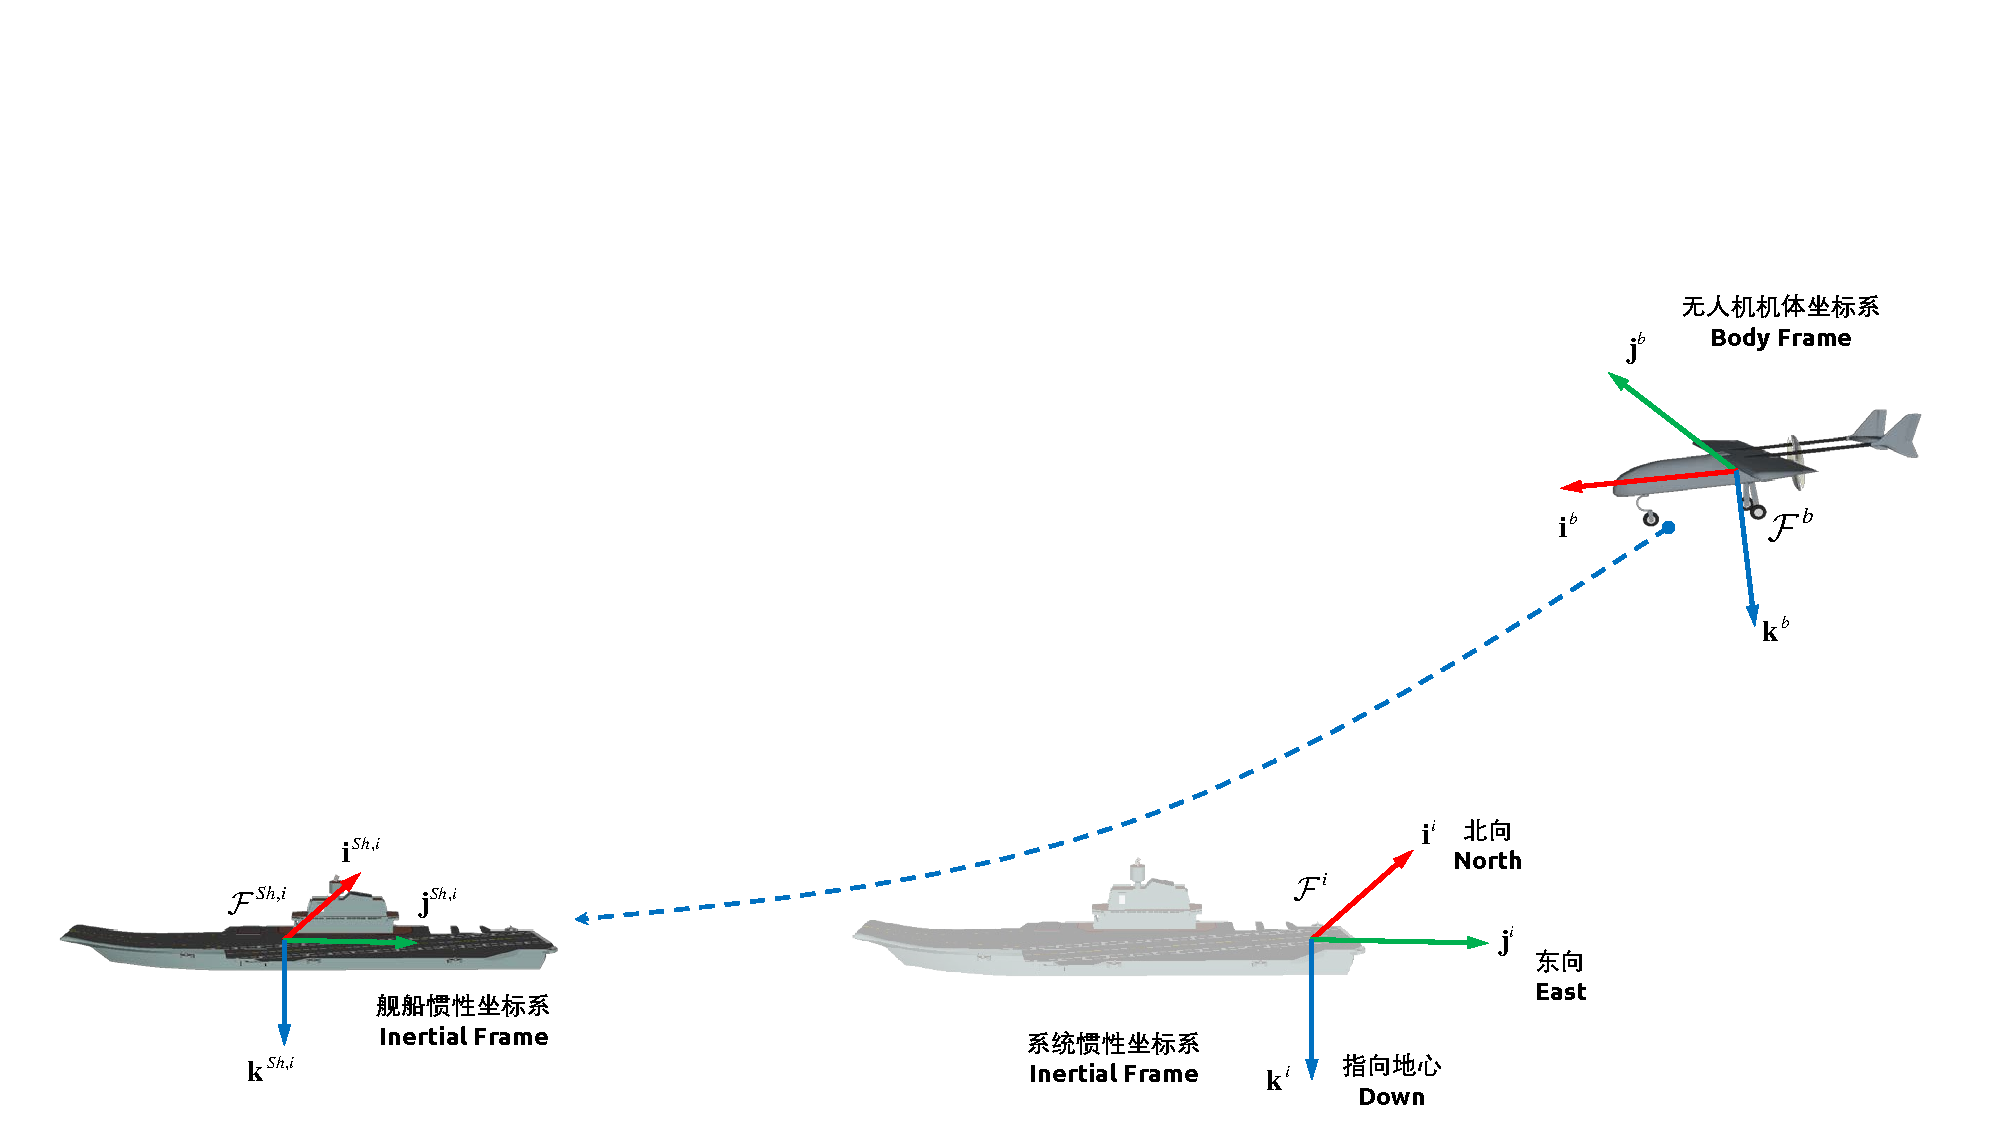
\includegraphics[width=\textwidth]{figs/chp02/chp02_01_sys_interial_frame.pdf}
	\caption{系统坐标系}
	\label{fig:_05}
\end{figure}

\subsection{无人机惯性坐标系}
无人机惯性坐标系($\mathcal{F}^v$,Vehicle Inertial Frame),该坐标系的原点位于飞机的重心,三轴方向与系统坐标系平行。

\begin{figure}[htb]   
	\centering
	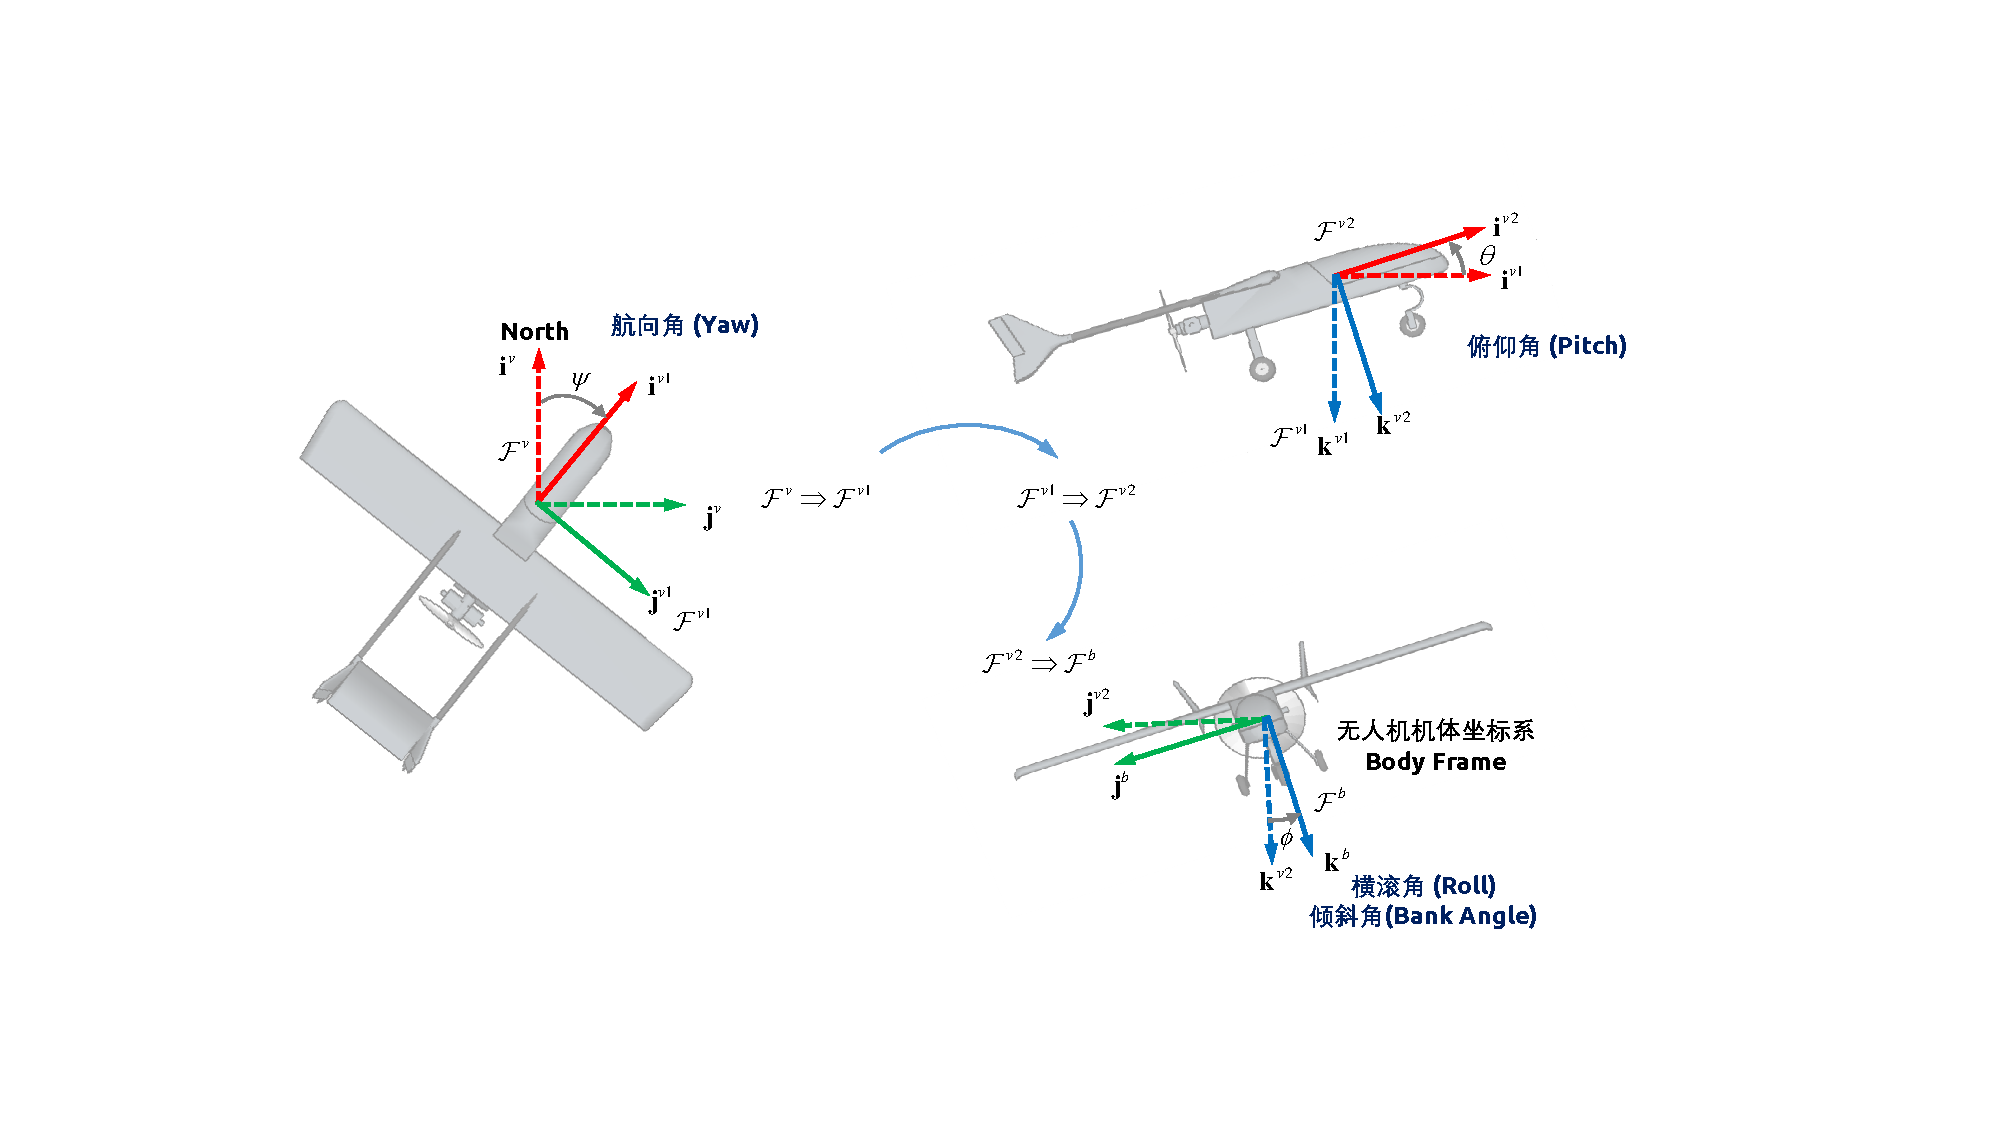
\includegraphics[width=\textwidth]{figs/chp02/chp02_02_uav_rpy.pdf}
	\caption{无人机机体坐标系与横滚角、俯仰角和偏航角定义}
	\label{fig:chp02_02_uav_rpy}
\end{figure}

无人机第一惯性辅助坐标系($\mathcal{F}^{v1}$ ),该坐标系绕无人机惯性坐标系$\mathbf{k}^v$轴按右手规则旋转得到,其中旋转角度定义为$\psi$,即偏航角(Yaw Angle)。

无人机第二惯性辅助坐标系($\mathcal{F}^{v2}$),该坐标系过绕人机第一惯性辅助坐标系$\mathbf{j}^{v1}$轴按右手规则旋转旋转得到,其旋转角度定义为$\theta$,即俯仰角(Pitch Angle)。

无人机机体坐标系($\mathcal{F}^b$,Body Frame ),该坐标系绕无人机第二惯性辅助坐标系$\mathbf{i}^{v2}$轴按右手规则旋转旋转得到,其旋转角度定义为$\phi$,即横滚角(Roll Angle),有时该角度也被称为倾斜角(Bank Angle)。

由机体惯性坐标系$\mathcal{F}^v$转换到机体坐标系$\mathcal{F}^b$的转换矩阵为
\begin{multline}
\mathcal{R}_v^b(\phi, \theta, \psi) =\mathcal{R}_{v2}^b(\phi)\mathcal{R}_{v1}^{v2}(\theta)\mathcal{R}_v^{v1}(\psi) \\
=\begin{bmatrix}
\cos \theta \cos \psi                             & \cos\theta \sin\psi                               & -\sin\theta         \\
-\cos\phi \sin\psi + \sin\phi \sin\theta \cos\psi & \cos\phi \cos\psi + \sin\phi \sin\theta\sin\psi   & \sin\phi \cos\theta \\
\sin\phi \sin\psi + \cos\phi \sin\theta \cos\psi  & -\sin\phi \cos\psi + \cos\phi \sin\theta \sin\psi & \cos\phi \cos\theta
\end{bmatrix}
\end{multline}


机体坐标系$\mathcal{F}^b$转换到稳定坐标系$\mathcal{F}^s$的转换矩阵为
\begin{equation} 
\mathcal{R}_b^s(\alpha) = \begin{bmatrix}
\cos \alpha                             & 0                               & \sin \alpha         \\
0 & 1   &0 \\
-\sin \alpha   & 0 & \cos \alpha
\end{bmatrix}
\end{equation}

稳定坐标系$\mathcal{F}^s$转换为风坐标系$\mathcal{F}^w$的转换矩阵为
$$
\mathcal{R}_s^w(\beta) = \begin{bmatrix} \sin \beta  & \cos \beta  &  0      \\  - \sin \beta & \cos \beta   &0 \\  0   & 0 &1  \end{bmatrix}
$$

风坐标系$\mathcal{F}^w$转换为机体坐标系$\mathcal{F}^b$转换矩阵为

$$
\mathcal{R}_w^b (\alpha,\beta) = \begin{bmatrix} \cos \beta \cos \alpha & - \sin \beta \cos \alpha  & - \sin \alpha      \\	 \sin \beta & \cos \beta   & 0 \\	\cos \beta   & -\sin \beta \sin \alpha & \cos \alpha \end{bmatrix}
$$

\subsection{无人机稳定坐标系}
无人机稳定坐标系($\mathcal{F}^s$,Stability Frame),该坐标系绕无人机机体坐标系$\mathbf{j}^b$按左手规则旋转得到。其中,定义无人机相对于机体周边空气的速度向量为$\mathbf{V}_a$,其大小为$V_a$。为使机翼产生升力,机翼与风速的夹角必须为正,该角度定义为攻角。这里使用左手系的原因是为更方便的定义定义攻角$\alpha$的正负,即沿稳定坐标系$\mathbf{j^s}$按右手系转动到机体坐标系的角度为正。稳定坐标系的$\mathbf{i}^s$轴与空速向量$\mathbf{V}_a$在$\mathbf{i}^b$-$\mathbf{k}^b$的投影方向平行。


\begin{figure}[htb]   
	\centering
	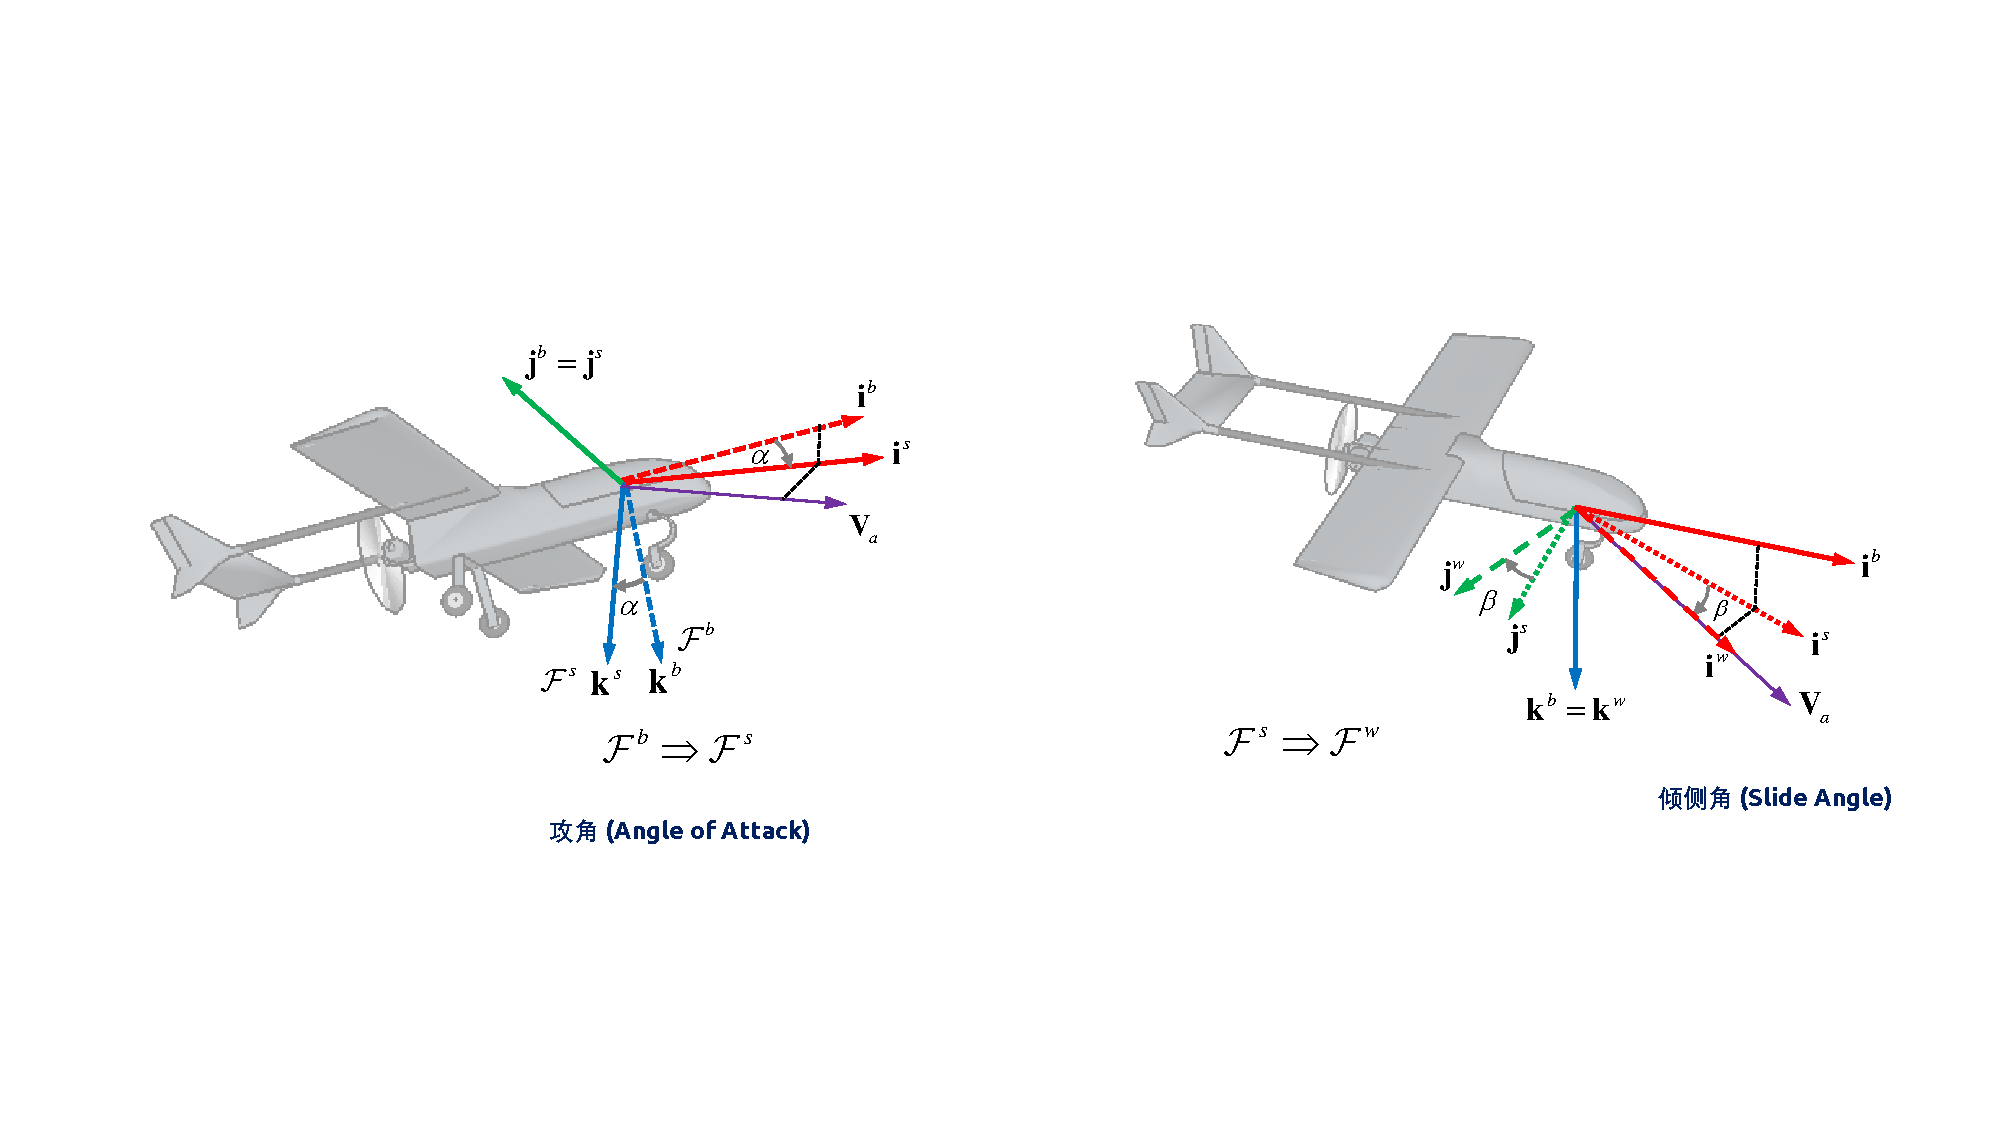
\includegraphics[width=\textwidth]{figs/chp02/chp02_03_uav_aoa_bank.pdf}
	\caption{无人机稳定坐标系与攻角、侧滑角定义}
	\label{fig:chp02_03_uav_aoa_bank}
\end{figure}

\subsection{无人机风向坐标系}
无人机风向坐标系($\mathcal{F}^w$,Wind Frame),该坐标系的$\mathbf{i}^w$轴与风速方向相同,可以通过旋转稳定坐标系的$\mathbf{k}^s$轴$\beta$角度得到,该角度$\beta$被定义为侧滑角。
\begin{figure}[htb]   
	\centering
	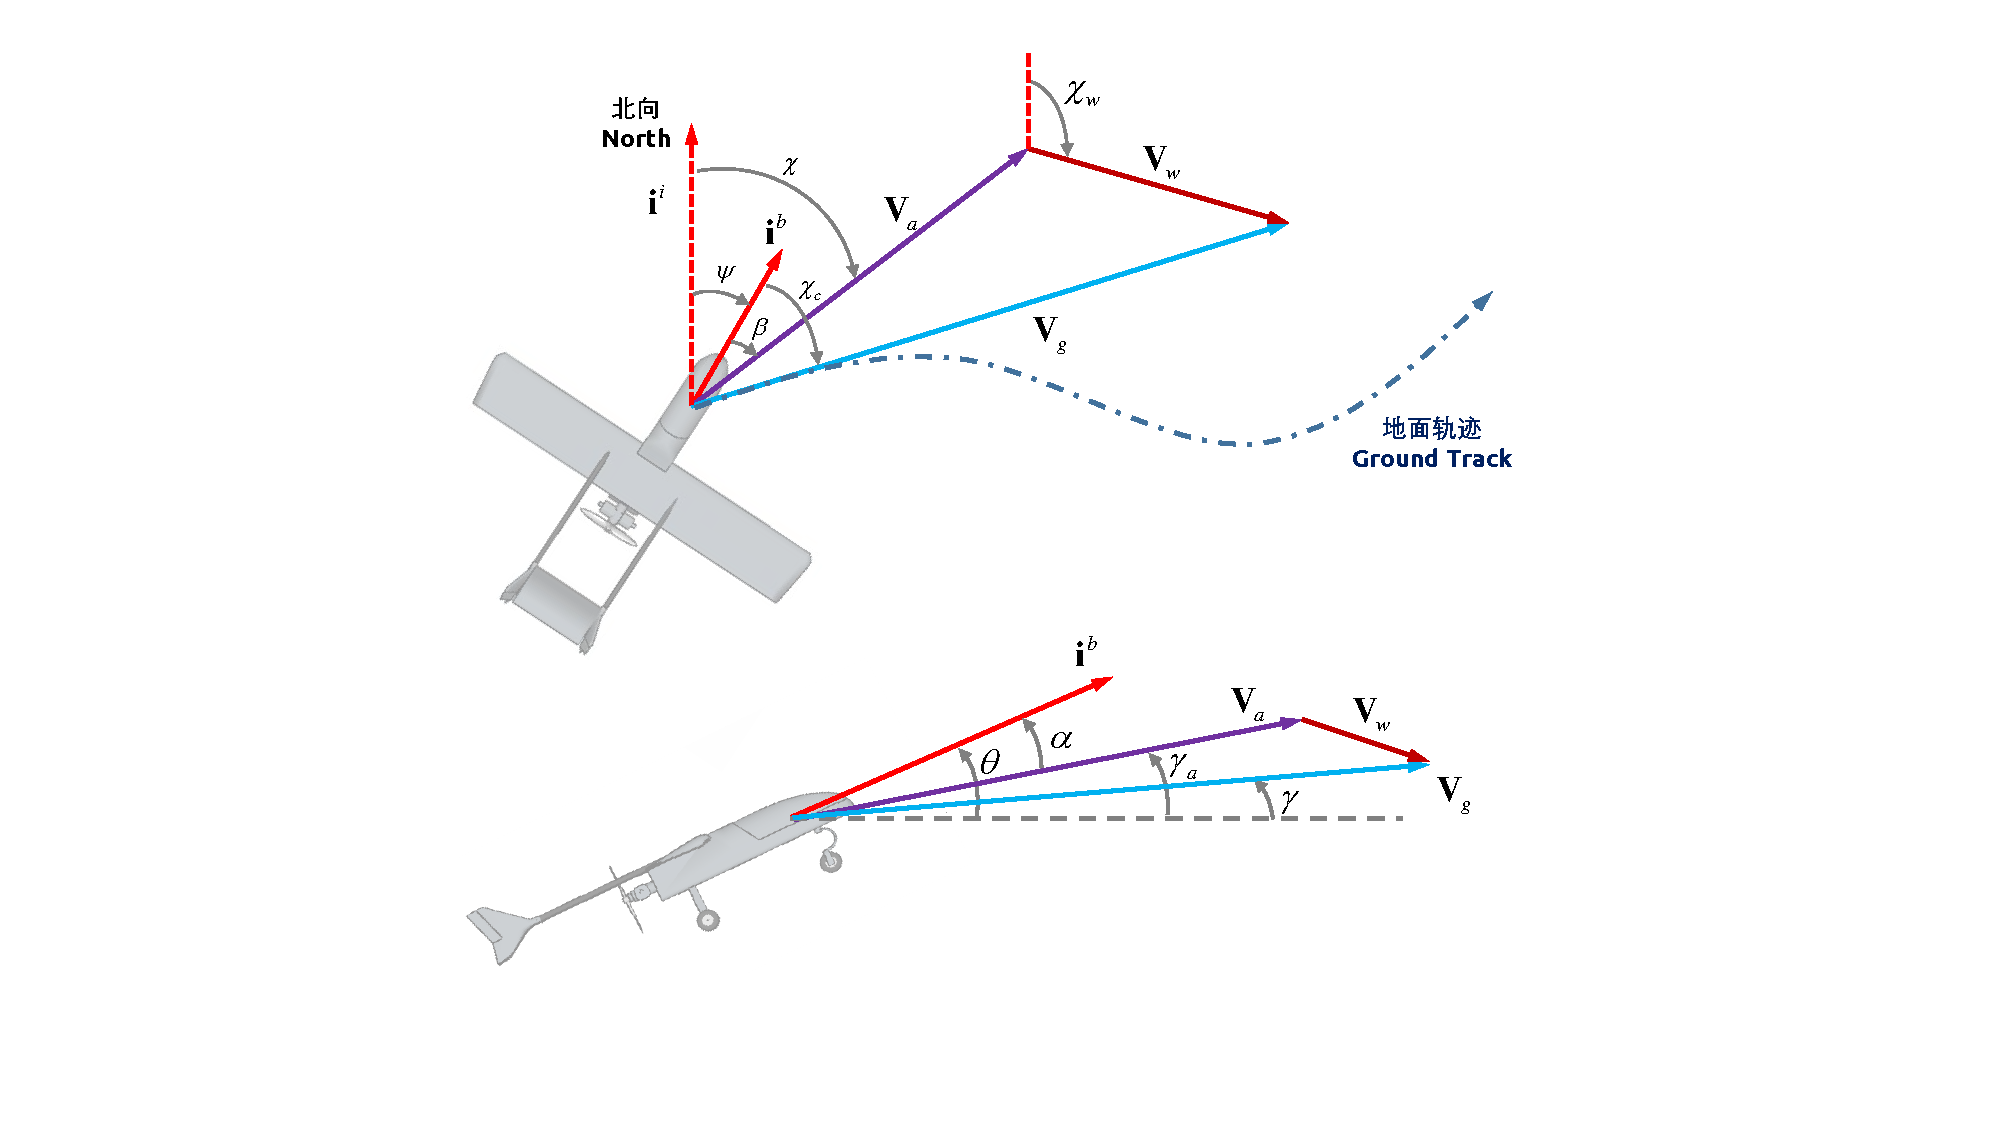
\includegraphics[width=0.8\textwidth]{figs/chp02/chp02_04_uav_wind_frame.pdf}
	\caption{无人机惯性坐标系}
	\label{fig:chp02_04_uav_wind_frame}
\end{figure}



\subsection{无人机轨迹坐标系}
\begin{figure}[htb]   
	\centering
	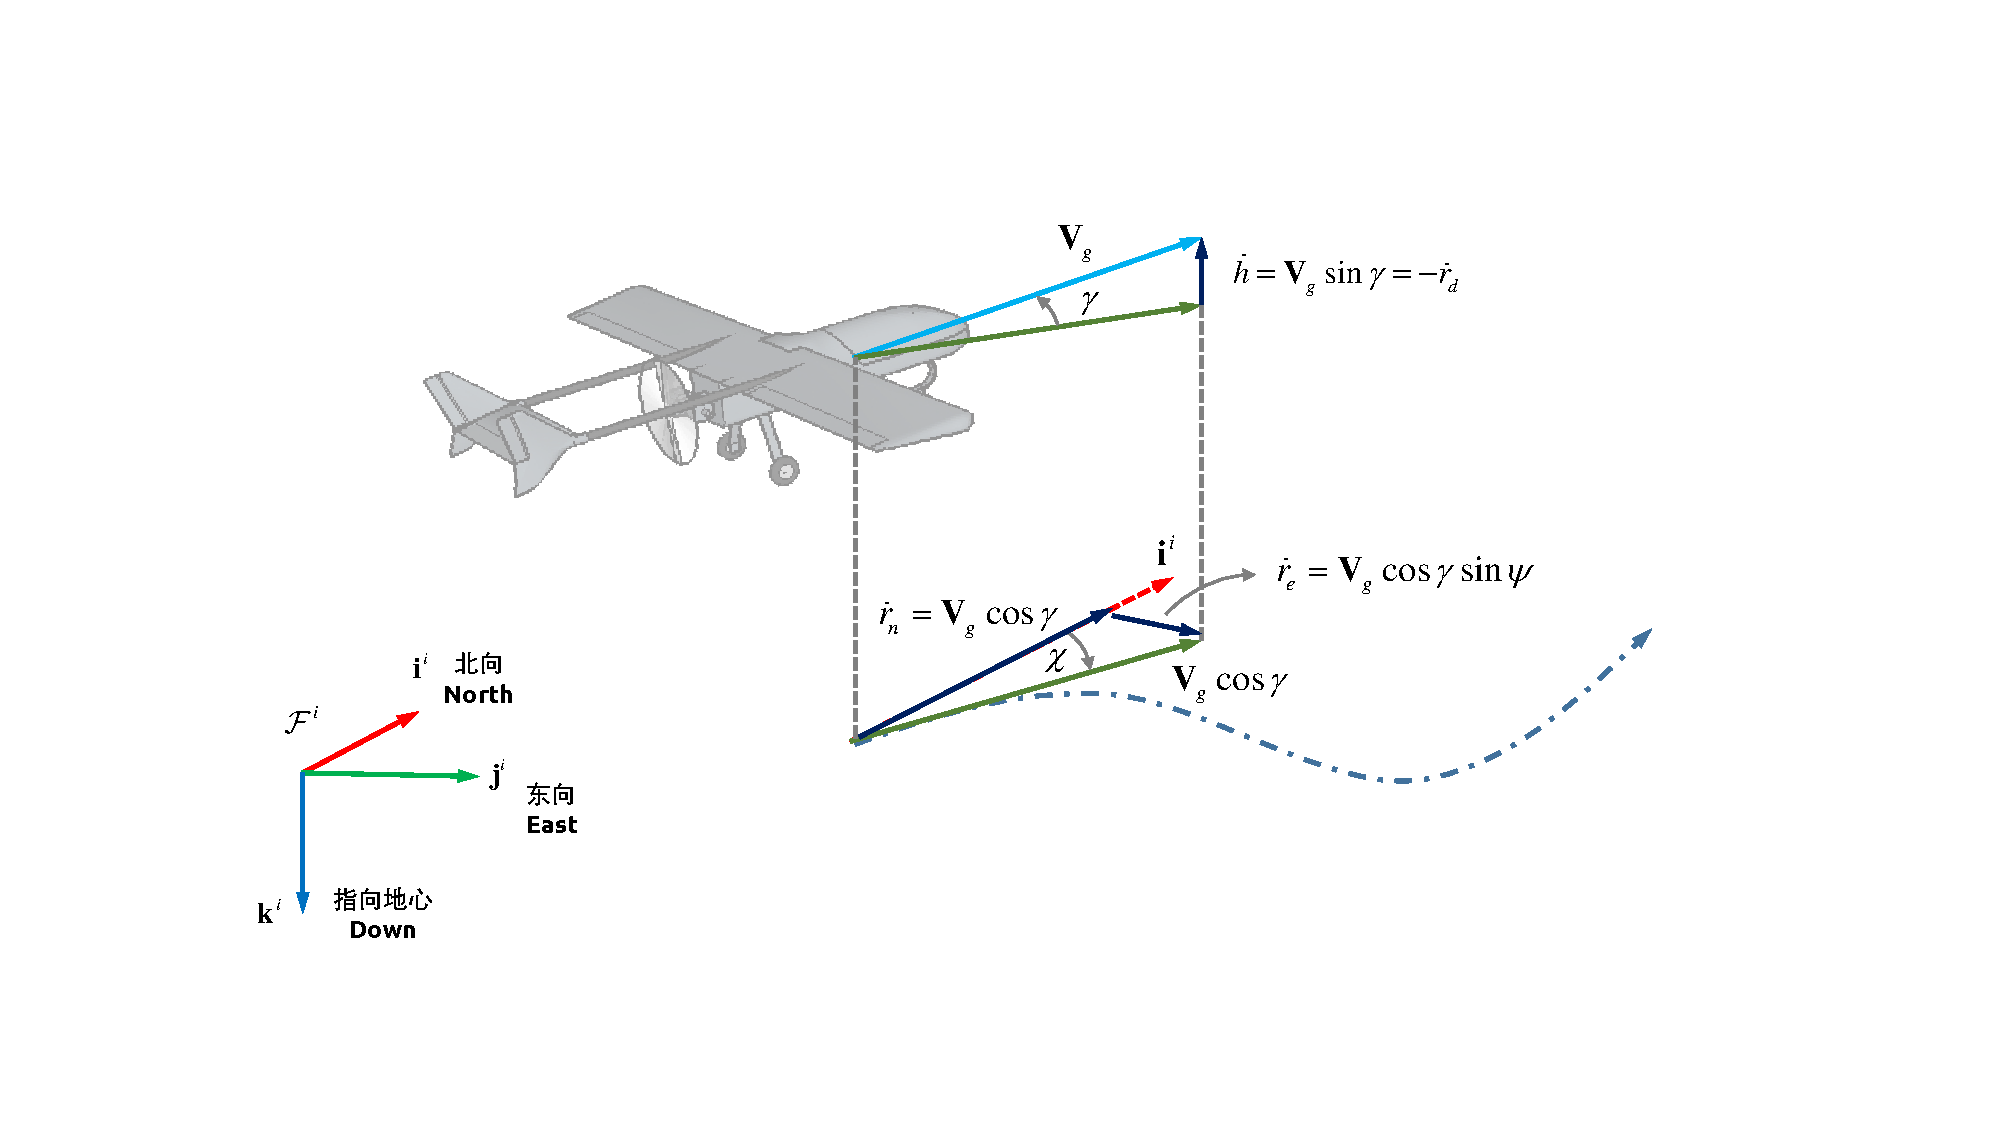
\includegraphics[width=0.8\textwidth]{figs/chp02/chp02_05_uav_course_frame.pdf}
	\caption{无人机惯性坐标系}
	\label{fig:chp02_05_uav_course_frame}
\end{figure}



\section{舰船系统坐标系定义}

\begin{figure}[htb]   
	\centering
	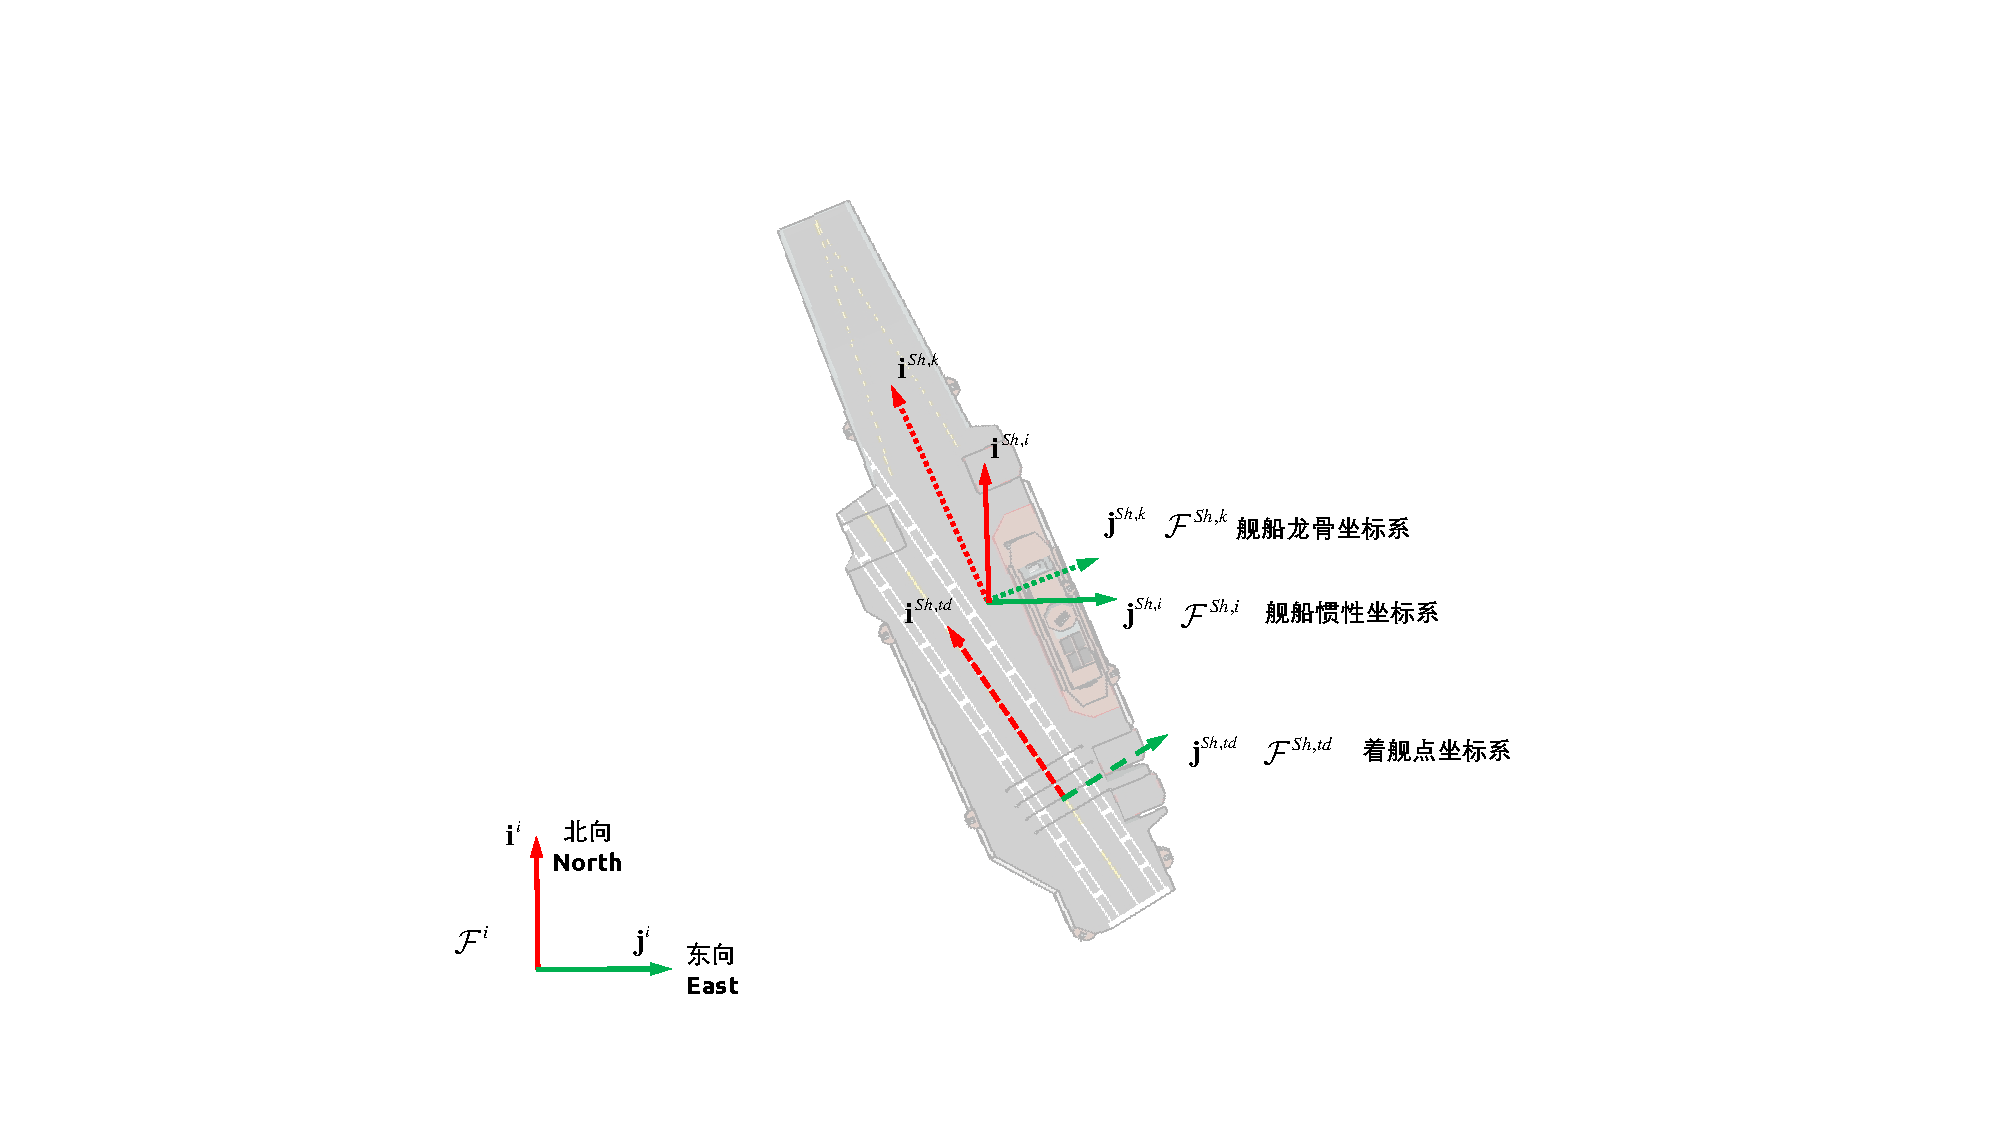
\includegraphics[width=0.8\textwidth]{figs/chp02/chp02_08_ship_interial_frame.pdf}
	\caption{无人机惯性坐标系}
	\label{fig:chp02_08_ship_interial_frame}
\end{figure}


\begin{figure}[htb]   
	\centering
	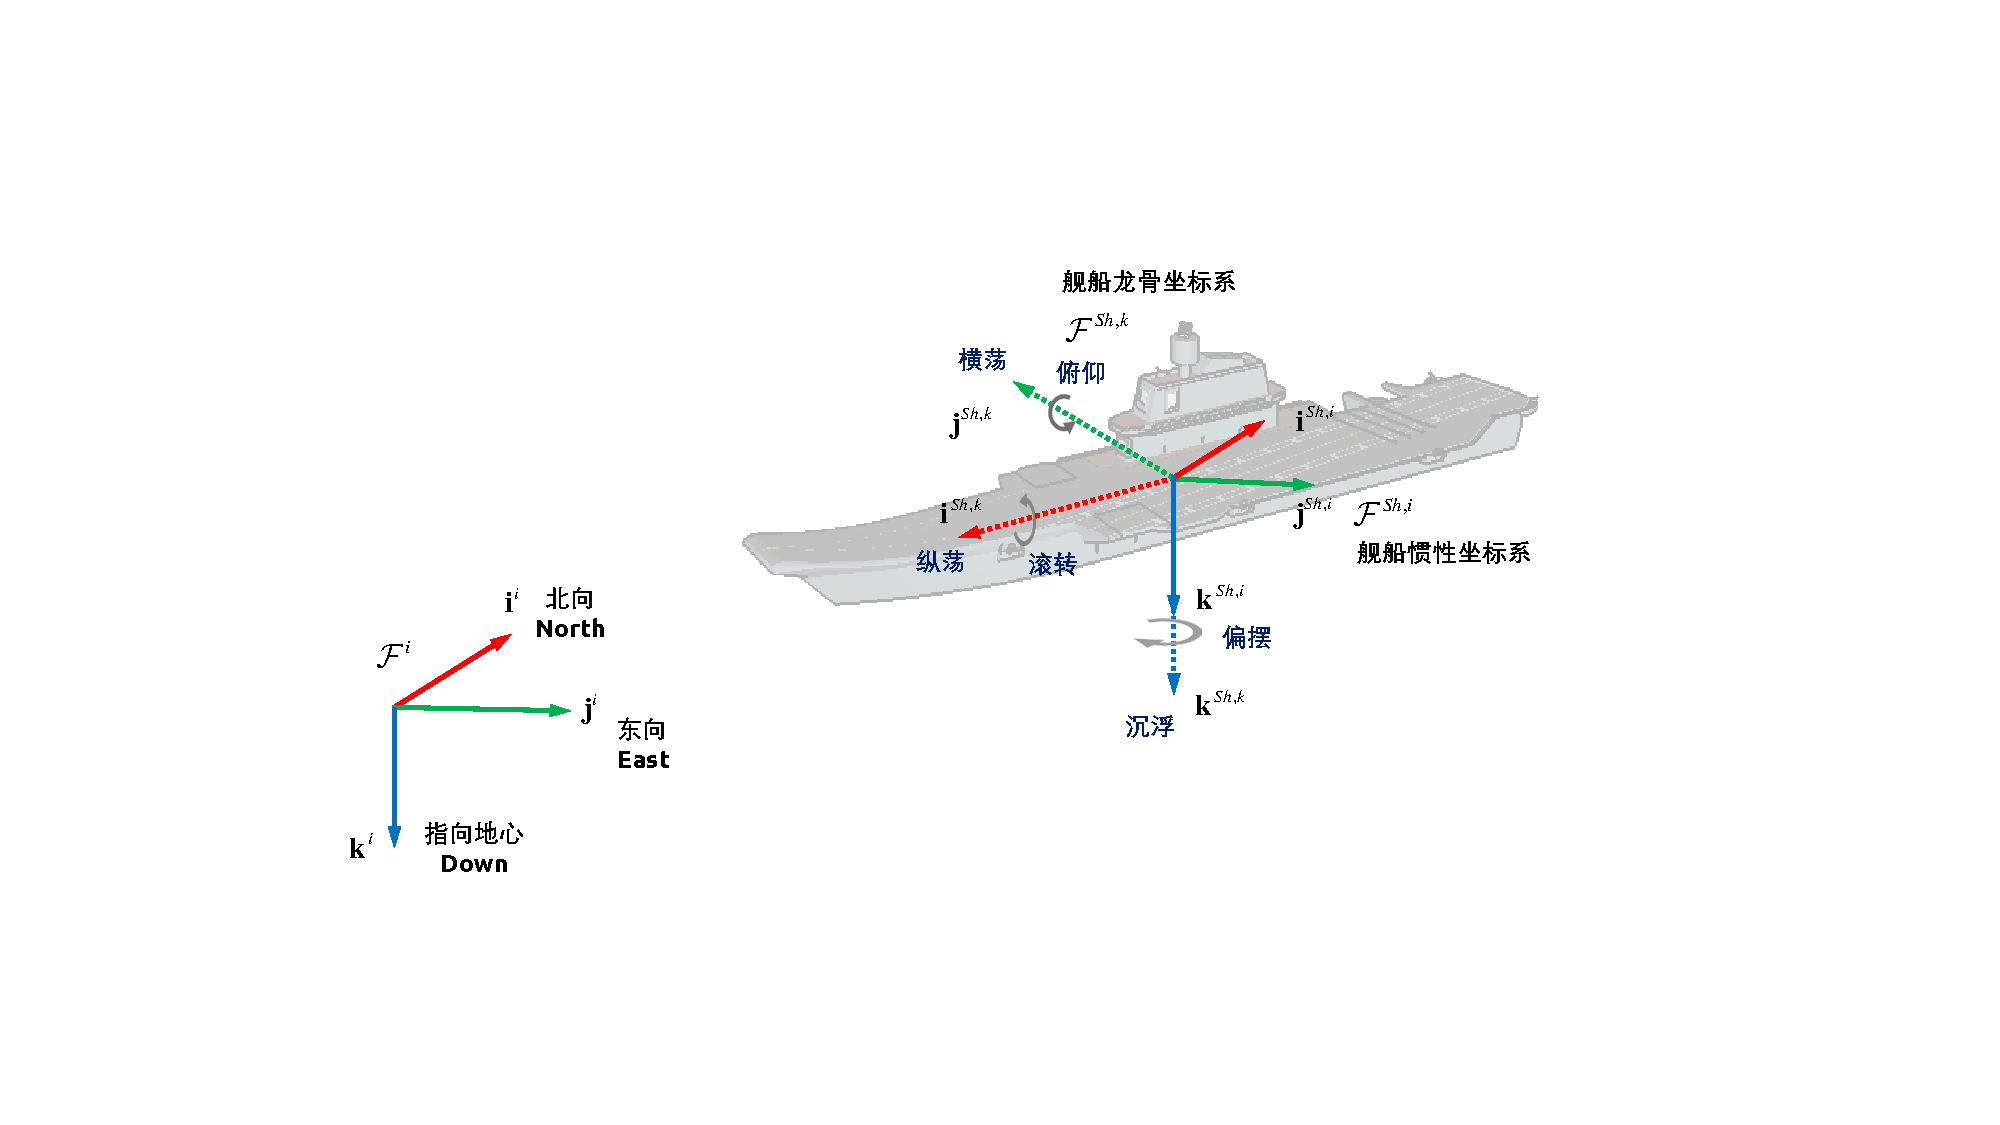
\includegraphics[width=\textwidth]{figs/chp02/chp02_09_ship_motion_frame.pdf}
	\caption{无人机惯性坐标系}
	\label{fig:chp02_09_ship_motion_frame}
\end{figure}


\section{舰载引导系统坐标系定义}
 
